\section{Extra Experiments}
Further experiments were conducted with an increased dimensionality, specifically within
the range of $100 < k <= 300$. The results indicate a consistent trend, with no discernible
turning point. The patterns previously reported continue to persist and, if applicable,
move towards a convergence point.

Furthermore, a series of $p$ values within the range of $0.5 < p < 2$ were examined,
focusing on the \emph{Avg} statistics values. Notably, the \emph{Avg Variance} revealed
novel insights, as detailed in~\autoref{sec:variance}. A distinct pattern shift
was observed in the \emph{Avg Variance} corresponding to $p={1,2}$, transitioning from
an increasing trend to a decreasing one. Upon investigating intermediate $p$ values
(1.7, 1.9, and 1.95), it was discovered that the transition point may initiate at $p=1.95$.
This is where the \emph{Avg Variance} pattern begins to slightly decrease as the dimensionality,
denoted by $k$, increases.

\begin{figure*}[ht!]
    \centering
    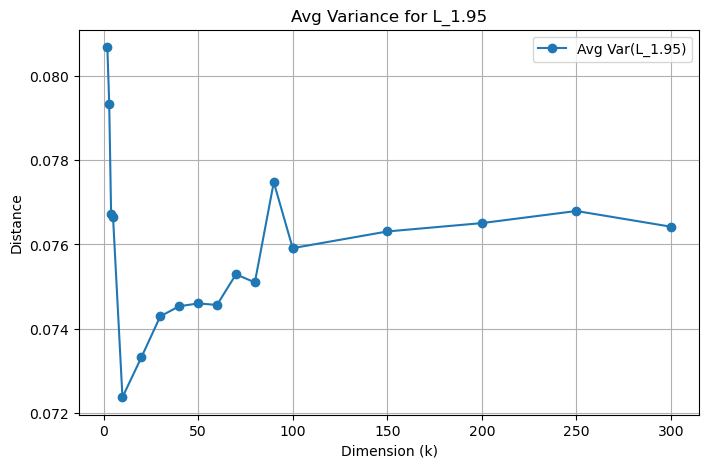
\includegraphics[width=0.8\textwidth,height=\textheight,keepaspectratio]
    {lp-turning-point.png}
    \caption{\emph{Avg Variance} for $L_{1.95}$}\label{fig:lp-turning-point}
\end{figure*}
